\chapter{Memory}
\label{ch:memory}

Store the 32-bit word \code{0x12345678} at address 8. What does address 8
contain afterward? The answer is not the whole word. A0 memory gives each
address one byte, so the store must distribute the four bytes across four
addresses. To define that one instruction, we need an address, a width, a byte
order, a valid range, and a rule for failure.

Memory makes order matter twice. The bytes of one value have an order across
addresses, and separate accesses have an order through time.

It also makes absence observable. A register read always names one of A0's
eight registers. A memory access can form a word address for which some needed
byte does not exist. The semantics must decide that failure before it can
state what the instruction writes.

\section{A finite map of bytes}

\begin{definition}[title={A0 data memory}]
A0 \keyterm{data memory} is a finite map from \(w\)-bit addresses to bytes. A
load reads \(w/8\) consecutive addresses and joins their bytes in
little-endian order. A store splits a \(w\)-bit word and writes its bytes to
consecutive addresses in that order.
\end{definition}

Object \obj{A0.def.memory} records the complete contract. This is data memory,
not the immutable program map. An A0 store cannot overwrite instruction bytes
in the first model.

\subsection{Addressable memory separated place from meaning}

Early calculating machines had storage, but not every store presented the
same abstraction. A value might live in a physical register, a delay line, a
drum position, or a location selected by wiring. The stored-program idea
made numbered locations serve both instructions and data. Later machines
varied the physical technology while preserving a stable architectural
question: what value does a load obtain from a named address?

That question contains two separations. First, an address names a place, not
a type. The byte at address 8 does not announce whether it belongs to an
integer, a character, a pointer, or an instruction. The operation that reads
the byte supplies the width and interpretation. Second, architectural memory
is not a photograph of the hardware. Caches, translation structures, buses,
and storage cells may participate in an access without appearing as separate
components in the instruction-set state.

A0 begins below both companion architectures with a finite byte map. The map
is deliberately small enough to draw and complete enough to define loads,
stores, overlap, and failure. It has no page table, cache, permission bit,
memory-mapped device, or concurrent writer. Those omissions let us establish
the sequential byte rules first. Chapter 16 will ask what must change when a
later model admits the missing mechanisms.

\begin{archive}[title={The durable abstraction is a numbered place}]
Memory technology has changed repeatedly. The architectural contract survives
by naming locations and the effects of accessing them, rather than requiring
software to describe the physical device that retains each bit. That
abstraction is powerful precisely because it has a boundary: timing and
concurrent visibility need additional rules.
\end{archive}

An access of \(n=w/8\) bytes beginning at address \(a\) is valid only when all
addresses \(a,a+1,\ldots,a+n-1\) belong to the finite data-memory range. The
first A0 model permits an access to begin at any address; it imposes no data
alignment restriction. That is a design choice, not a claim about either
companion architecture.

Address arithmetic still uses words. The machine forms a memory address by
adding the sign-extended eight-bit offset to a base register modulo \(2^w\).
It then checks the resulting sequence of byte addresses against the finite
range. Wraparound arithmetic does not make an out-of-range byte valid.

\begin{keyidea}[title={Address formation and access validity are different rules}]
Word arithmetic always produces an effective-address word. A memory access
succeeds only when every byte in its declared range exists. The first fact
does not imply the second.
\end{keyidea}

The requirement that every byte exist prevents a dangerous half-definition.
If a four-byte access begins at a valid address but ends beyond memory, A0
does not improvise a shorter access. The requested width belongs to the
instruction form. Either the whole access completes or the state records a
trap.

\subsection{Memory equality is checked one address at a time}

Two finite memories are equal when they have the same domain and return the
same byte at every address in that domain. Their construction history does not
matter. One memory may have reached its present contents through a store;
another may have begun with those bytes. If every lookup agrees, the A0 state
cannot distinguish them through memory.

This pointwise definition gives memory proofs a reliable shape. To show that
two stores produce equal memories, choose an arbitrary address and divide the
argument according to whether it lies inside or outside each write footprint.
To show that memories differ, one address with unequal bytes is enough. The
first task is universal; the second needs a witness.

\begin{example}[title={One byte separates two memories}]
Let memories \(M_1\) and \(M_2\) share the domain 0 through 15. Suppose they
agree everywhere except address 9, where \(M_1(9)=\mathtt{00}\) and
\(M_2(9)=\mathtt{01}\). An eight-bit load at 9 distinguishes them directly.
A thirty-two-bit little-endian load at 8 also distinguishes them because the
unequal byte receives weight \(2^8\).
\end{example}

Preservation claims use the same definition. Saying that a store changes only
its requested range means that every address outside that range returns its
old byte. The phrase \emph{everything else is unchanged} is therefore not a
gesture toward the rest of memory. It abbreviates a quantified clause that a
checker must test or derive.

\section{Store, then load}

Return to \code{0x12345678}. Its little-endian split is
\code{78}, \code{56}, \code{34}, \code{12}. A store at address 8 writes
\code{78} at 8, \code{56} at 9, \code{34} at 10, and \code{12} at 11. A
load from address 8 joins those four bytes with weights
\(2^0,2^8,2^{16},2^{24}\).

\begin{figure}[htbp]
\centering
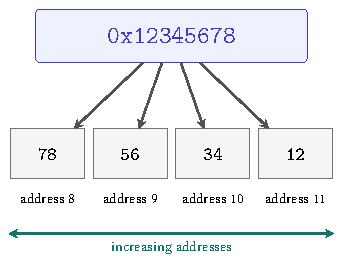
\includegraphics[width=0.78\textwidth]{figures/little-endian-store}
\caption{A little-endian store places the low-weight byte at the lowest
address. The word's printed hexadecimal order and memory's address order run
in opposite visual directions here.}
\figalt{The word 0x12345678 splits into bytes 78, 56, 34, and 12 at addresses 8 through 11.}
\label{fig:little-endian-store}
\end{figure}

The word has not been numerically reversed. The low byte receives the low
address. Endianness describes the relation between byte addresses and place
values.

\subsection{Bytes acquire a value through an access rule}

Memory stores bytes. A load instruction decides how many adjacent bytes to
read and how to place them in its result. The four locations in
Figure~\ref{fig:byte-sequence-readings} therefore support several valid
readings. An eight-bit load uses one byte. A sixteen-bit load uses the first
two. A thirty-two-bit load uses all four. None changes the stored bytes.

\begin{figure}[htbp]
\centering
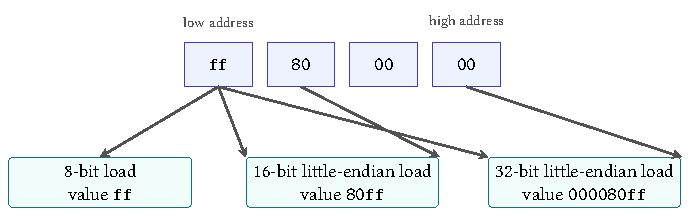
\includegraphics[width=0.88\textwidth]{figures/byte-sequence-readings}
\caption{A byte sequence does not carry one compulsory width. The selected
load form determines the range and the little-endian place values.}
\figalt{Four bytes ff, 80, 00, and 00 lead to separate eight-bit, sixteen-bit, and thirty-two-bit load results.}
\label{fig:byte-sequence-readings}
\end{figure}

The destination width creates a further question. A narrow load into a wider
register must say what fills the upper bits. Zero extension fills them with
zero. Sign extension repeats the narrow value's high bit. Loading the byte
\code{ff} into a thirty-two-bit destination can therefore produce
\code{000000ff} or \code{ffffffff}. Endianness alone chooses neither result.

\begin{definition}[title={Load interpretation}]
A load interpretation consists of a starting address, a byte count, a byte
order, and a rule for placing the assembled value in the destination. The
last rule includes any zero extension, sign extension, truncation, or
preservation of destination bits.
\end{definition}

This definition prevents a common shortcut. Saying that a machine is
little-endian settles the weights of bytes within a multi-byte value. It does
not settle the access width, destination width, signed extension, alignment,
or failure behavior. Two instruction forms can read the same first byte and
still produce different register values without disagreeing about byte order.

Stores reverse the construction but have their own width. A byte store writes
one low byte even when its source register is wider. A word store writes the
declared sequence of bytes. Unwritten neighboring bytes retain their old
values. This preservation fact is the memory version of the frame conditions
from Chapter 2, and later proofs will rely on it as heavily as on the bytes
that change.

The round-trip proof now has a machine premise. Let \(x\) be a \(w\)-bit word
and suppose every address in the \(w/8\)-byte range beginning at \(a\) is
valid. The store writes
\[
  b_i=\bigl(x\mathbin{\mathrm{div}}2^{8i}\bigr)\bmod 2^8
\]
at address \(a+i\). The following load reads that same \(b_i\) and computes
\[
  \sum_{i=0}^{w/8-1} b_i2^{8i}.
\]
Chapter 1 showed that these disjoint byte positions join to \(x\). No other
memory byte enters the sum. The load therefore returns \(x\).

\begin{proofkit}[title={\iconProofKit\ Store then load}]
The proof has three premises: the store and load use the same width, the same
starting address, and a wholly valid range. The store writes byte \(b_i\) at
\(a+i\). The load reads that same location and multiplies the byte by
\(2^{8i}\). Chapter 1's split/join identity reconstructs \(x\). If any premise
changes, the conclusion needs a new argument.
\end{proofkit}

Notice what the proof does not require. It does not require the starting
address to be a multiple of four, because the first A0 memory model permits
unaligned data access. It does not require unrelated bytes to have any
particular value. It does require the store to be atomic on failure and no
intervening write to change the loaded range.

The valid-range premise is load-bearing. Suppose a four-byte store begins at
the last address of memory. Only its first target address exists. A0 traps and
leaves data memory unchanged; it does not perform a one-byte fragment of the
store. A later load cannot appeal to the round-trip argument because the
required store never completed.

\begin{warning}[title={Partial failure changes the theorem}]
A faulty implementation might write each valid byte and trap only when it
reaches the missing address. That route changes memory before reporting
failure. It does not implement A0's atomic store rule, and a later observation
of the valid prefix can expose the difference.
\end{warning}

\begin{figure}[htbp]
\centering
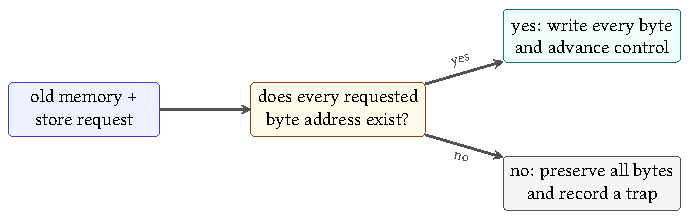
\includegraphics[width=0.86\textwidth]{figures/atomic-store-outcomes}
\caption{A0 checks the complete store range before selecting either a full
memory update or a trapped state with memory preserved. There is no partial
commit between them.}
\figalt{An old memory and store request reach a complete-range test, which leads either to writing every byte or preserving all bytes and trapping.}
\label{fig:atomic-store-outcomes}
\end{figure}

Atomic here describes one transition in the sequential A0 semantics. It means
that a failing store has no partly updated successor. It does not claim the
stronger hardware property that another processor can never observe pieces of
a successful multi-byte store. A0 has no second processor or concurrent
observer. Reusing the word outside that scope would quietly add a theorem the
model cannot even state.

The success case has a frame rule. Let \(A\) be the set of addresses written
by a valid store, let \(M\) be the old memory, and let \(M'\) be the result.
For every address \(d\) outside \(A\),
\[
  M'(d)=M(d).
\]
Inside \(A\), the corresponding source byte determines \(M'(d)\). Together,
the inside and outside clauses define the entire new finite map. A checker
that compares only the requested range verifies the first clause and misses
corruption elsewhere.

The trap case has an even stronger frame rule: every memory address retains
its old byte. Other state changes also require an explicit decision. A0
records the trapped outcome and does not advance into another instruction.
The source and destination registers remain as the step rule states. A real
architecture may record exception metadata in additional state; that state is
outside A0 rather than implicitly preserved by it.

\begin{example}[title={A control that reverses the weights}]
A faulty load joins the bytes from addresses 8 through 11 with address 8 at
weight \(2^{24}\) instead of \(2^0\). It returns \code{0x78563412}, not
\code{0x12345678}. The stored bytes are individually correct. The relation
between address and weight is wrong.
\end{example}

\section{Effective addresses and range}

For the A0 operand \([r_1-4]\), the base is the word \(R[r_1]\), and the
offset is the sign extension of the immediate byte \code{fc}. The effective
address is their width-\(w\) sum. Only after forming that word does the machine
check whether the whole access range exists.

This order separates two ideas that are easy to blur. Word arithmetic always
produces a word, even when it wraps. Memory validity is a predicate on the
resulting addresses. If an eight-bit base contains 2 and the offset is -4, the
effective address is 254. A four-byte access still traps in a memory whose
valid range is 0 through 63.

The address expression also does not identify a fixed location by itself.
Changing \(R[r_1]\) changes the address denoted by \([r_1-4]\). Operand syntax
and state work together to select bytes.

The valid range may itself wrap in word arithmetic. A width-eight access of
four bytes starting at 254 names the word addresses 254, 255, 0, and 1 if we
apply modular addition to each address. A0 does not infer validity from that
cycle. Its finite memory domain must contain every address the access rule
names. This makes the finite map, rather than the maximum word value, the
authority for presence.

Nor must a finite domain be one uninterrupted interval. A model may contain
addresses 0 through 31 and 48 through 63 while leaving a hole between them.
A four-byte access beginning at 30 then finds its first two bytes and misses
its last two. Checking that 30 and 33 fit within the minimum and maximum
domain addresses would accept the access incorrectly. The semantics asks
membership for each requested address.

That generality is useful even when an implementation later chooses a dense
array. The mathematical interface describes which addresses exist. A dense
representation can add a lemma that its bounds check is equivalent to
per-address membership. A sparse representation can check the map directly.
The theorem belongs to the interface; the faster check earns its place by
establishing equivalence to that theorem.

\begin{tryit}[title={Form first, check second}]
At width eight, evaluate base 250 with offsets 5, 6, and 10. For each result,
state the effective-address word and then test a four-byte access against a
memory domain containing addresses 0 through 255. Repeat with a domain
containing only addresses 0 through 63.
\end{tryit}

\subsection{A range is a set of byte addresses, not two unchecked endpoints}

For a non-wrapping access, it is convenient to write the requested range as
the right-exclusive interval \([a,a+n)\). It contains \(a\) through \(a+n-1\)
and contains exactly \(n\) addresses. Right-exclusive intervals compose cleanly: an
access ending at \(b\) and one beginning at \(b\) are adjacent rather than
overlapping.

The notation must not hide word wrap. If \(a+n\) is calculated modulo
\(2^w\), the two endpoints alone no longer reveal whether the access crossed
the maximum word. A valid-range checker should enumerate the declared byte
positions or use an arithmetic condition that detects overflow before relying
on an interval comparison. Testing only that the first and last words belong
to a domain can also fail when the finite domain has a hole between them.

Alignment adds an independent predicate. A rule may require
\(a\bmod n=0\), a weaker alignment, or none. Passing that test does not make
the range present. Failing it may trap even when every byte exists. Thus a
complete access rule has at least three stages: form the effective-address
word, check address-policy predicates such as alignment, and check every byte
needed by the transfer.

This separation becomes useful when relating machines. A0 permits an
unaligned access that a selected real-ISA environment may reject. The real
operation cannot refine the A0 operation on all A0 states without either
restricting the input relation to aligned addresses or representing the
additional failure in the abstract model. Matching successful examples does
not repair the missing case.

\section{When two accesses meet}

Two memory accesses \keyterm{alias} when their byte ranges overlap in the same
state. Equality of their starting addresses is sufficient but not necessary.
A four-byte access at \(a\) and another at \(a+2\) share addresses \(a+2\) and
\(a+3\).

\begin{figure}[htbp]
\centering
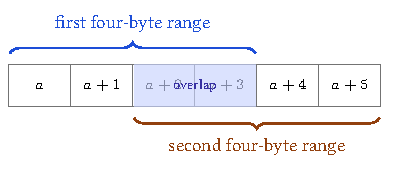
\includegraphics[width=0.84\textwidth]{figures/aliasing-ranges}
\caption{Equal starting addresses are not required for aliasing. These
four-byte ranges share two addresses.}
\figalt{Ranges a through a+3 and a+2 through a+5 overlap at a+2 and a+3.}
\label{fig:aliasing-ranges}
\end{figure}

Let the first store write \code{0x11111111} at \(a\), and let the second write
\code{0x22222222} at \(a+2\). In that order, the bytes at \(a\) through
\(a+5\) end as
\[
  \mathtt{11}\quad\mathtt{11}\quad\mathtt{22}\quad
  \mathtt{22}\quad\mathtt{22}\quad\mathtt{22}.
\]
Reverse the stores and the middle two bytes become \code{11}. The final memory
differs even though each store, considered alone, writes the same source word.

Disjoint stores have a simpler argument. If their address ranges share no
byte, the first store changes no address read or written by the second, and
the second changes no address written by the first. At every address, either
one designated store supplies the final byte or the original byte remains.
The final data memories are therefore equal after either order, provided both
accesses are valid and neither traps.

Overlap breaks the disjointness step. A proof that exchanges memory operations
must establish non-aliasing, account for the shared bytes, or accept a narrower
claim. A register identity alone supplies none of these.

\begin{proofkit}[title={\iconProofKit\ Why disjoint stores commute}]
Choose any address \(d\). If \(d\) lies in the first range, disjointness says
the second store does not change it; the first store supplies the same final
byte in either order. The symmetric case handles the second range. If \(d\)
lies in neither range, both stores preserve its original byte. The cases cover
the memory domain, so the final maps are equal. Validity is required so that
both orders perform both complete stores.
\end{proofkit}

The address-by-address proof explains exactly why the theorem stops at
overlap. An address in both ranges has two possible final writers, and their
order decides which one wins. We may recover commutation when the overlapping
bytes happen to be equal, but that is a different premise and a narrower
theorem.

\subsection{Loads turn aliasing into a data dependence}

Place a load beside a store. If their ranges are disjoint and both operations
succeed, moving the load before the store preserves the loaded value. The
store changes no byte read by the load. If the ranges overlap, the loaded
value may contain old bytes in one order and new bytes in the other. This is a
memory dependence even when the instructions name different starting
addresses or use different widths.

The proof again works address by address. For every byte position read by the
load, non-aliasing says the store preserves that memory entry. The join rule
therefore receives the same byte at every weight in both executions. Equal
input bytes give an equal loaded word. The argument also needs the same
outcome in both orders: moving an access across a trap can change whether the
other access occurs at all.

Aliasing is state-dependent when addresses come from registers. The printed
operands \([r_1]\) and \([r_2+4]\) neither guarantee overlap nor rule it out.
A compiler may establish non-aliasing from an input contract, an allocation
rule, or arithmetic facts about the registers. Without such evidence, treating
different syntax as different memory is wishful typesetting.

Widths make the question asymmetric. A one-byte load inside a four-byte store
range aliases the store, while a neighboring one-byte load may not. A proof
must compare byte footprints rather than the source-language types or the
number of registers written. This is why later instruction semantics will
record read and write footprints separately.

\begin{keyidea}[title={Memory dependence follows byte footprints}]
Two accesses interact when the bytes read or written by one meet the bytes
written by the other. Mnemonics, operand spellings, and unequal starting
addresses are not enough to decide the question.
\end{keyidea}

\section{Memory in the two companion machines}

The later RV64 slice will use distinct load and store forms to move values
between integer registers and memory. Arithmetic in the selected base forms
uses registers. An effective address commonly combines one base register with
an immediate.

The later x86-64 slice will include selected arithmetic forms that name a
memory source or destination. Such a form can combine address calculation,
memory access, and arithmetic in one decoded instruction. Its semantic rule
must still expose the address, bytes, value width, state effects, and possible
exception.

This comparison holds one question fixed: which included instruction forms
may access memory? It does not say that every instruction in one architecture
has one character or that a shorter assembly spelling has fewer semantic
obligations.

For either slice, a usable memory rule must answer the same checklist. It must
name the address inputs, byte range, value construction, alignment premise,
successful state change, and failure outcome. The answers may differ. The
questions do not.

Both real architectures live inside systems that add translation and access
policy. A program commonly supplies a virtual address. Hardware and operating
system state determine whether that address names storage, whether the access
is permitted, and which exception follows a failure. Device mappings may give
a read or write effects unlike ordinary memory. None of this turns the byte
order question into a page-table question; it adds layers around the transfer.

The book's selected scalar slices will make those layers explicit by premise
or exclusion. A theorem about an ordinary mapped region should say so. A
decoder theorem need not model translation because it concerns bytes already
supplied to decoding. A program theorem that loads from memory cannot borrow
that simplification without naming how the bytes become available.

This discipline prevents an architectural manual from doing more work than it
actually does. The manual specifies instruction behavior and exceptions in a
declared mode. An application binary interface may add stack and object-layout
conventions. An operating system supplies mappings and policies. A language
implementation adds rules about valid objects and undefined behavior. A proof
crossing these layers needs a relation between them, not a single citation to
the lowest one.

\begin{table}
\centering
\caption{Memory questions that syntax alone cannot answer.}
\begin{tabular}{p{0.24\textwidth}p{0.56\textwidth}}
\toprule
Question & Required semantic fact \\
\midrule
Where? & effective-address calculation and width \\
How much? & access width and byte range \\
Which value? & byte order and extension or truncation \\
What changes? & destination, memory, program counter, and other state \\
What can fail? & alignment, range, permission, or selected architectural outcome \\
\bottomrule
\end{tabular}
\end{table}

\section{The implementation boundary}

The Axeyum state and memory package must implement the finite map, valid-range
check, atomic load and store outcomes, little-endian split and join, wrapped
effective-address calculation, and observations of changed and unchanged
bytes. Object \obj{OP.a0.state-memory} records that obligation.

Its negative controls are already suggested by the chapter. Reverse the byte
weights. Permit a range whose last byte is absent. Partly modify memory before
a trapped store. Declare two overlapping ranges disjoint. Each mutation must
be rejected by the corresponding check.

The introductory Axeyum route should make memory visible rather than burying
it in a solver formula. A reader constructs a finite memory map, performs one
store, inspects the changed bytes, and loads the word back. The route then
asks for a counterexample to the round trip under the printed validity
premise. Any model returned by the solver must replay through those executable
store and load functions.

The controls should travel through the same route. Reversing the join weights
must yield a concrete unequal-byte witness. Removing the last address from the
domain must produce a trap and unchanged memory. A partial-write mutation must
fail an observation of the valid prefix. These checks test different
boundaries; one passing control cannot stand in for the others.

The artifact for one memory step should bind the complete old state, decoded
instruction, effective address, requested footprint, outcome, and complete new
state. A compact list of changed bytes is useful for display, but the checker
must reconstruct the full successor and confirm the frame rule. Otherwise an
artifact can omit an illicit change and still look like a plausible diff.

At the Python layer, the introductory exercise should expose values a reader
can inspect without duplicating semantics. The reader supplies bytes and an
initial state, calls the bound Rust implementation, and receives a structured
step record. Python may print the address calculation and memory table. It
must not recompute the successor with a second informal implementation and
call agreement with itself a check.

The first solver question can stay finite and sharp: for every width-eight
word and every valid four-byte starting address in a declared finite domain,
does storing and then loading return the word while preserving every byte
outside the range? A counterexample must replay through executable memory
operations. A no-counterexample result needs an evidence route that covers
the whole stated domain. Until that package exists in Axeyum, the object
records an implementation obligation rather than a machine-backed result.

\begin{sidebar}[title={Why a memory formula is not yet memory semantics}]
A formula that expands four byte variables can establish a relation among
those variables. It does not by itself establish address formation, finite
range checking, atomic failure, or preservation of unrelated bytes. The A0
memory package must connect all of those rules before later instruction proofs
may depend on it.
\end{sidebar}

The store/load result in this chapter is a reader proof under a printed
premise. It does not stand in for the absent executable memory model. Once that
model exists, the round trip and each bad variant must run through the same
memory semantics used by later instruction proofs.

Memory has made sequence visible. Two individually valid stores can leave
different final states when their order changes. A list of instructions still
does not tell us which one runs next. For that we need a program counter, a
program, and a trace through both.

\section{Exercises}

\begin{enumerate}
\item \textbf{Execute.} Store \code{0x89abcdef} at address 4 in little-endian
order. List the four writes and reconstruct the loaded word by hand.
\item \textbf{Break.} Reverse the byte weights in the load rule. Give the
smallest two-byte word for which the faulty round trip differs from the
original, and calculate both results.
\item \textbf{Prove.} Prove that two valid stores to disjoint byte ranges
commute. State exactly where the argument fails for overlapping ranges.
\item \textbf{Transfer.} For one later RV64 load form and one selected x86-64
memory-source form, list the address inputs, value width, destination, and
possible exceptional outcome that their pinned semantics must supply.
\item In eight-bit address arithmetic, compute the effective address for base
2 and offset -4. Explain separately why the word result exists and why a
four-byte access may still be invalid.
\item Design an atomicity control for a four-byte store whose final address is
outside memory. State which bytes a faulty partial store would change and what
A0 requires instead.
\item \textbf{Execute.} Draw the two ranges in
Figure~\ref{fig:aliasing-ranges}. Perform the two example stores in both
orders and list the final byte at every address from \(a\) through \(a+5\).
\item \textbf{Break.} Change A0 so a failing store writes its valid prefix.
Give a pre-state and an observation that distinguish the faulty result from
the required atomic trap.
\item \textbf{Prove.} Strengthen the disjoint-store argument to one load and
one store: state a non-aliasing premise under which moving the load before the
store preserves the loaded value.
\item \textbf{Transfer.} Explain why a real-ISA memory form needs both a
source-pinned address rule and a source-pinned failure model before it can
refine the A0 access, even when a sample address calculation matches.
\end{enumerate}
